\documentclass{llncs}

\usepackage{amssymb}
\usepackage{amsmath}
\setcounter{tocdepth}{3}
\usepackage{graphicx}
\usepackage{url}
\usepackage{mdwlist}
\urldef{\mailsa}\path|{xsongx, tingwang}@nudt.edu.cn|
\newcommand{\keywords}[1]{\par\addvspace\baselineskip
\noindent\keywordname\enspace\ignorespaces#1}

\begin{document}

\mainmatter  % start of an individual contribution

% first the title is needed
\title{Dividing for Combination: Semi-supervised Sentiment Classification for Microblogs}
%
% a short form should be given in case it is too long for the running head
%\titlerunning{Lecture Notes in Computer Science: Authors' Instructions}
\author{Xie Songxian%
%\thanks{Please note that the LNCS Editorial assumes that all authors have used
%the western naming convention, with given names preceding surnames. This determines
%the structure of the names in the running heads and the author index.}%
\and Wang Ting}
%
%\authorrunning{Lecture Notes in Computer Science: Authors' Instructions}
\institute{Department of Computer Science and technology, School of Computer,\\
National University of Defence Technology,
Changsha, China\\
\mailsa\\
\url{http://www.nudt.edu.cn}}

%\toctitle{Lecture Notes in Computer Science}
%\tocauthor{Authors' Instructions}
\maketitle

\begin{abstract}
Sentiment analysis is the computational study of how opinions(positive or negative) are expressed in language. It has been an important research area of Natural Language Processing in recent years.
There are many challenges for sentiment analysis especially of the social media language. 
This paper focuses on context dependence, which has been the most challenging problem, and proposes a novel framework to solve the problem.
By dividing the feature space into two parts, a general classifier on general part of features is trained on off-the-shelf labelled idiom resources, and a context classifier on context-dependent part of features is trained on random tweets retrieved from microblogs in distant supervision manner. 
Then a semi-supervised framework is developed to combine the general classifier and context classifier into a bootstrapping classifier. 
Experiments results show that the proposed framework is effective and achieves encouraging accuracy performance. 
\keywords{sentiment analysis; idioms; general classifier; context classifier;microblog}
\end{abstract}

\section{Introduction}
\label{intro}
Sentiment analysis is the computational study of how opinions, attitudes, emotions, and perspectives are expressed in language. 
Sentiment analysis provide tools and techniques for extracting subjective information from large datasets and summarizing it for successive application such as Business Intelligence, Public Opinion Analysis, and Election Prediction, etc\cite{xsongx:b1}. 
Sentiment classification, which deals with determining sentiment orientation of target text, is the classification form of sentiment analysis\cite{xsongx:b2}. 
Although it can be viewed as a special text categorization problem, in fact sentiment classification is a more challenging task than text classification, because sentiment expressions critically depend on domains and context\cite{xsongx:b6}.

With the emergence and prosperity of social networks, the amount of user-generated content (UGC) has risen exponentially over the last decade, and such content is now always at our fingertips.
Mircoblog is one of the most important social networks which has absorbed millions of users to update their status (conventionally called tweets in microblog) day and night.
Beyond merely displaying news and reports, the mircoblog itself is also a large platform where different opinions are presented and exchanged. 
Users comment, discuss, compliment, argue and complain over topics they are interested in, sharing their own feelings publicly. 
It has been well recognized that UGC of microblog with rich sentiment information can trigger more attention, feedback or participation, and sentiment analysis researchers have begun to pay more and more attention to microblogs content \cite{DBLP:conf/hicss/StieglitzD12}.
The distillation of subjective knowledge from such abundant language resources becomes an important part of applications in fields such as commerce, tourism, politics and health. 
But as a freely-publishing platform, users may use or create new words of abbreviations and acronyms that seldom appear in conventional text documents, for example, words like "coooooool", “OMG",":-(", are intuitive and popular in microblog.
Though they may provide convenience for on-line communications of users, it is difficult for computer to accurately identify the semantic meanings of these words. 
To make situation worse, new words may arise and old words may change their meaning continuously in tweets.
The noisy quantity, informal nature and explosive vocabulary of tweets make sentiment classification of tweets a very difficult and challenging task, because the sentiment in tweets often depends on such particular expressions as emoticons, repeated letters and exclamation, etc., which get their semantic meaning only in the context of microblogs. 
Context dependence has been the main challenge sentiment classification of tweets must face.
In this work, we have focused on the context-dependent problem of sentiment classification on microblogs. 

To solve the problem, we propose a novel semi-supervised framework based on our two rational hypotheses.
Firstly the problem is formulated as feature vector space model of text classification. 
By dividing the feature space into two parts, a general classifier on general part of features is trained on off-the-shelf labelled idiom resources, and a context classifier on context-dependent part of features is trained on tweets randomly retrieved from microblogs in distant supervision manner. 
Then a semi-supervised framework is developed to combine the general classifier and context classifier into a bootstrapping classifier. 
The experiments carried out on a Chinese microblog platform show that the framework is  effective and achieves encouraging accuracy performance.

The rest of the paper is organized as follows: Related works are discussed in Section~\ref{related}. Our two hypotheses are put forward in
Section~\ref{problem}, and our framework of semi-supervised sentiment classification is described in Section~\ref{framework}. The results and discussions of the experiment are presented in Section~\ref{experiment}. Finally we conclude about our work in Section~\ref{conclusion}.
\section{Related Works}
\label{related}
The task of sentiment analysis has been a popular research area for years. 
Previous efforts mainly focuses on reviews and news comments. 
Generally, in terms of methodology, rule-based approaches and machine-learning based approaches are two major popular methods, and the machine-learning based approaches usually act as an upper bound for other methods to compare with, in that they have higher performance because of the strong generalization ability of classifiers\cite{xsongx:b1,xsongx:b4}.

Recently, sentiment analysis researchers have begun to pay more and more attention to the massive user-generated content of social networks such as Twitter\footnote{\url{twitter.com}}. 
Many studies showed that the unique characteristics of Twitter can be incorporated into sentiment analysis techniques.
Barbosa and Feng~\cite{Barbosa:2010RSD} first investigated to use a two-stage Support Vector Machine (SVM) classifier for tweets sentiment classification which proved to be robust regarding biased and noisy data. 
Hu et al.~\cite{Hu:2013www} interpreted emotional signals available in social media data for unsupervised sentiment analysis by providing a unified way to model two main categories of emotional signals: emotion indication and emotion correlation. 
Jiang et al.~\cite{xsongx:b6} focused on target-dependent Twitter sentiment classification, they proposed to improve target-dependent Twitter sentiment classification by taking both target-dependent features and related tweets into consideration. 
Wang et al.~\cite{Wang:2011TSA} focused their study on hashtag-level sentiment classification, they proposed a novel graph model and further improved the model using an enhanced boosting classification setting. 
Amir Asiaee T et al.~\cite{AsiaeeT:2012} presented a cascaded classifier framework for per-tweet sentiment analysis by extracting tweets about a desired target subject, separating tweets with sentiment, and  setting apart positive from negative tweets.
Hu et al.~\cite{Hu:2013ESR} extracted sentiment relations between tweets based on social theories, and proposed a novel sociological approach to utilize sentiment relations between messages to facilitate sentiment classification and effectively handle noisy Twitter data.
Motivated by sociological theories arguing that humans tend to have consistently biased opinions, Guerra et al.~\cite{CalaisGuerra:2011BOT} addressed challenges of topic-based real-time sentiment analysis by proposing a novel transfer learning approach with a suitable source task of opinion holder bias prediction.
Thelwall et al.~\cite{Thelwall:2010SSS,Thelwall:2012SSD} designed SentiStrength, an algorithm for extracting sentiment strength from informal English text. The algorithm built on human-evaluated dictionaries for words connotated with positive or negative sentiments and exploited the grammar and spelling styles in typical microblogs.
Zhao et al.~\cite{Zhao:2012UTM} presented a hierarchical generative model, called user-sentiment topic model (USTM) used in social network analysis to find influential users on topic level with sentiment information.

All works above have tried to adapted their methods to the microblogs by making use of the network and language characteristics, no matter what approaches they have taken. However, in this paper, we solve the context-dependent problem from a novel perspective by separating context-independent part of features from context-dependent part of features of sentiment classification.
\section{Problem Formulation and Solution}
\label{problem}
\subsection{Problem Formulation}
\label{formulation}
Simply speaking, sentiment classification aims to classify text as predefined sentiment polarity classes(negative or positive).  
Formally, Given document corpus $ D=\lbrace d_{1},\dots ,d_{n} \rbrace$ , and predefined sentiment classes $ C=\lbrace 1,-1\mid \mathrm{positive}=1,\mathrm{negative}=-1 \rbrace$ , the task of sentiment classification is to predict each $ d_{i} $ with a label $ c_{i} $. 
To be along with text categorization, each document can be represented as a vector of features $ x=\bbbr^{n} $, where $ n $ is the size of a pre-specified feature volume $ V $. 
For sentiment classification, the weight of each entry in the vector usually is often specified as binary, with weight equals to 1 for feature present in the vector and 0 for absent. 
Given a training dataset $ X=\lbrace x_{1},\dots,x_{m} \rbrace $, a classifier can be build:
\begin{equation}
\label{e1}
  f:X \longrightarrow Y, Y=\lbrace 1,-1 \rbrace \enspace .
\end{equation} 
and employ it to predict label for an unseen instance $ x $ by computing $ f \left( x \right)   $, with each instance represent as a vector $ x=\left( w_{1},\dots,w_{v} \right)  $, in which $ w_{i} $ is the $ i $th feature’s weight. 
\subsection{Feature Space Division}
\label{division}
In previous sentiment classification researches, there is an underlying hypothesis, which implies all features in the text vector represent the document’s sentiment polarity equally. 
In fact, some features may only appear in specific context, while others appear across any context. 
As an example, an English tweet is listed as following:

\textit{@Kid\_Cloudz: Happy birthday to Yessicaaaa! :D lovee you feggit wish you the best day everrrrr!!!!! @030268.}

If simple "bag-of-words" features are considered, all words would be extracted as equal features to model the sentiment when computationally classifying sentiment polarity of this tweet. 
However with thorough considerations, we can find that such words as "@Kid\_Cloudz, :D, lovee, everrrrr,!!!!!" are mainly used in the  language context of microblogs, while "Happy, birthday, wish, best, thanks" are sentiment indicators of text almost in any language context. 
With such intuition, we proposed a feature space division hypothesis as:
\spnewtheorem{hypothesis}{Hypothesis}{\bfseries}{\rmfamily}
\begin{hypothesis}
\label{h1}
In the feature space of sentiment classification, features can be divided into two different parts:
\begin{itemize*}
\item context-independent part, i.e. general features, which are indicators of sentiment independent of any language context;
\item context-dependent part, i.e. context features, which indicate sentiment in specific language context.
\end{itemize*}
\end{hypothesis}
Formally, for the text feature vector of a tweet $ x=\left(  w_{1},\dots,w_{l},w_{l+1},\dots,w_{v} \right) $, it could be divided into two parts:
\begin{equation}
\label{e2}
x=\left\{
\begin{array}{rcl}
x_{g}     & \qquad        &:\mbox{general features}\\
x_{c}     &  \qquad       &:\mbox{context features}
\end{array}
\right. \enspace .
\end{equation}
where $ x_{g}= \left( w_{1},\dots,w_{l}\right) $ denotes the general part of feature space, while $ x_{c}= \left( w_{l+1},\dots,w_{v}\right) $ denotes the context dependent part.

Based on Hypothesis~\ref{h1}, we studied following questions in this paper:
\begin{itemize*}
\item How to identify each divided part of features, and what does it mean to the 
sentiment classification of tweets? 
\item How to model sentiment of tweet with the two divided feature sets in 
the machine learning framework?
\item How to construct training dataset for sentiment classifiers based on 
the two parts of features separately?
\end{itemize*}
\section{Sentiment Classification Framework}
\label{framework}
Besides traditional expressions, some languages of microblogs are often considered "Mars Language" because of their obscurity.  
However users could still distinguish the sentiment polarity of the tweet even if some words seem strange to them.
Intuitively, this kind of phenomenon may be explained by the general part of the tweet which is used to express the holistic sentiment polarity of the author across any context, and the polarity of general sentiment words are prone to be recognized by anyone independent of context knowledge. 
Comparably, for sentiment classification, we put forward that, the sentiment polarity of a document could sometimes still be recognized with only general part of feature space ($ x_{g} $ in Equation~\ref{e2}). 
That is to say, if general sentiment knowledge could be modeled, what sentiment polarity a tweet prefers for could still be classified based on such general sentiment models. 

In fact, many researchers have tried to establish all kinds of sentimental ontology lexicons to represent general knowledge of human’s sentiment, such as SentiWordNet~\cite{xsongx:b17} and General Inquiry~\cite{xsongx:b18} in English, Hownet\footnote{\url{http://www.keenage.com}}~\cite{xsongx:b19} and NTUSD~\cite{xsongx:b20} in Chinese, etc. 
However, some entries of these lexical resources have multiple senses with different sense representing different sentimental polarity, and the exact sentiment of each sense unavoidably depends on the context.
It seems a rather difficult task to find a general resources to model the context independent knowledge.
Actually such knowledge exists in many situations, and many regular language expressions in the form of one general phrase or combination of a few words could identify exact sentiment polarity independent of language context, such as idioms and proverbs. 
\subsection{General Sentiment Classifier}
\label{general}
There are many linguistic resources highly valuable for sentiment classification, of which idiom resources attract interests of this research. 
Idioms are common phenomena of many languages beside Chinese, such as ``castles in the air'', ``a bed of thorns'', and ``bring down the house'' in English.
The form of idioms is succinct and the meaning is penetrating, which is a quintessence part of the language. 
Generally speaking, the structure of idioms is fixed and can’t be changed at will, idioms have semantic intactness, which is not generally the simple summation of the literal meaning of each component, and most importantly, the sentimental polarity of idioms is independent and unchangeable under any context. 
There are many off-the-shelf idiom lexicons in all kinds of languages with entries taking the example form as:

\textit{castles in the air: a derogatory term, indicate the illusive things or impractical fanciness metaphorically.}

In this example, the entry is composed of three parts: the idiom ``castles in the air'', the semantic orientation ``a derogatory term'' representing negative
sentimental polarity and a short paraphrase with three general negative words (``illusive, impractical and fanciness''). 
The example provides us with a labelled sentimental instance with general sentiment features and a negative label.
Most importantly, the sentimental polarity of such instance is independent of any context just as the idiom it explains. 
Based on such observation, another hypothesis is proposed as follows:
\begin{hypothesis}
\label{h2}
The sentimental polarity of the idiom paraphrase is independent of language context just as the idiom it describes.
\end{hypothesis}
With Hypothesis~\ref{h2} admitted, we could constructed a training dataset with the features extracted from paraphrases of idioms as general feature vector, the sentimental polarity of idioms as sentimental labels. 
Then a context-independent classifier could be trained to model the general sentiment knowledge.
\subsection{Context Sentiment Classifier}
\label{context}
As the general sentiment features are only one part of all features in the whole feature space, the other context-dependent part of features should be considered in order to capture the subtle clues embedded in the specific sentiment expressions in language context of microblogs.
To model the context-dependent part of tweets, there are two questions must be solved. 
The first is to identify the context-dependent part of features extracted from tweets. 
In fact, new expressions appears on microblogs with the explosively increasing of UGC, which makes it rather difficult to clearly tell whether each word is context dependent or not. 
However tweets are conventionally short with the limitation of 140 characters, and users often express one particular sentiment in one tweet with a few words. 
Based on the particular characteristics of tweets, we make an assumption that if a tweet contains idioms,  sentimental polarity of words in a tweet are often context-dependent except for the idioms. 
The second is how to find labelled instances to train the context-dependent classifier. 
Some researchers have proposed distant supervision to solve the training data shortage of Twitter~\cite{xsongx:b36,xsongx:b37}. 
In this paper we establish our training dataset in a similar way.
We retrieve tweets on microblogs and try to get as many tweets as possible that contains idioms. 
By stripping off idioms, we extracted context-dependent features from left words, and took the sentimental polarity of idioms as labels. 
So we get our noisy labelled dataset and a context-dependent classifier is trained to model the context-dependent knowledge.
\subsection{Combination of Two Classifiers}
\label{combination}
Although theoretically the general classifier and context classifier could be able to model different sentiment knowledge separately and classify the sentiment of a tweet accurately to some extent, the coverage and efficiency of them are limited by the quality and quantity of training datasets. 
Besides, it is obvious that the paraphrase of idiom and tweet segments (lefts by stripping off idioms) is usually very short, so the feature vectors of datasets must be very sparse, which degrades the performance of the classifiers. 
For above reasons, a consistent bootstrapping machine learning framework is chosen to combine the two classifiers together. 
The framework is illustrated in Figure~\ref{fig1}. 
\begin{figure} 
\centering%
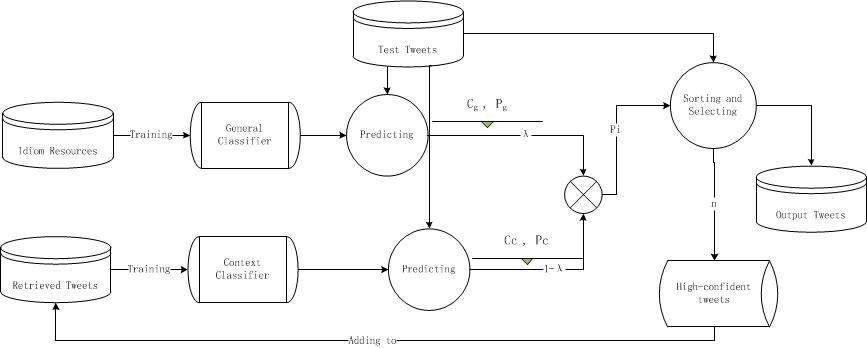
\includegraphics[width=5.0in,height=2.2in]{itse13.jpg}
\caption{The Bootstrapping sentiment classification Framework}
\label{fig1}
\end{figure}
As illustrated in the framework, in an iterating manner, the general classifier $ P_{g} $ and context classifier $ P_{c} $ are applied to test dataset so that the every test instance $ x_{i} $ is predicted labels $ c_{i}=\lbrace c_{g},c_{c}\rbrace $ initially, with confidence $ p_{i}= \lbrace p_{g},p_{c}\rbrace$. 
Then a combined confidence score is calculated with Equation~\ref{e3}:
\begin{equation}
\label{e3}
p_{i}=\left\{
\begin{array}{rcl}
\lambda\ast p_{g} + \left( 1-\lambda \right) \ast p_{c} \qquad \mbox{if} \quad c_{g}=c_{c};\\
0 \qquad \mbox{if} \quad c_{g} \neq c_{c};
\end{array}
\right. \enspace .
\end{equation}
where $ \lambda $ is the coefficient to control weights of different part of features. 
We initialize $ \lambda = 0.5 $ with equal weights of general part and context part of features, and to make combined classifier more adaptable for microblogs, we  increase the weight of context part step by step with the bootstrapping iteration progressing.
The test dataset initially labelled as $ c_{i} \left( c_{i} \in \lbrace 1, -1\rbrace \right)$ was sorted with descending confidence $ p_{i} $ for two sentimental categories $ C=\lbrace 1,-1\rbrace $ separately.
The $ n $  positive and negative instances with top high confidence are selected as new instances to add into the training dataset and improve the context classifier to a more context-aware classifier. 
Such a procedure iterates until convergence.
The output of such semi-supervised sentiment classification framework is the predicted results of test dataset. 
Above all, the whole framework could combine the two classifiers which constructed on divided feature space into a stronger classifier. 
\section{Classifier Description}
\label{classifier}
We adopt the same methods as Pang et al.~\cite{xsongx:b4}, in that they have applied Na\"\i ve Bayes, Maximum Entropy and Support Vector Machine classifiers to identify the effectiveness of machine learning techniques on sentiment classification, and they got satisfying result (accuracy of 82.9\%).
\subsection{Na\"\i ve Bayes Classifier}
\label{bayes}
Naïve Bayesian classifier is the most popular text classification techniques.
For sentiment classification problem as formulated in Section~\ref{formulation}, to determine which sentimental category $ c_{j} $ a document $ d_{i} $ belongs to, it is needed to compute the posterior probability $ P \left(c_{j} \mid d_{i} \right)$. 
According to the Bayesian probability and the multinomial model, based on the hypothesis that the probabilities of features $ w_{d_{i},k} $ are independent given document class, Equation~\ref{e4} is got:
\begin{equation}
\label{e4}
P \left(c_{j} \mid d_{i} \right) = \frac{P \left( c_{j} \right)\prod_{k=1}^{| d_{i} |} P \left( w_{d_{i},k} \mid c_{j} \right)}{\sum_{r=1}^{|C|}P \left( c_{r} \right)\prod_{k=1}^{| d_{i} |} P \left( w_{d_{i},k} \mid c_{r} \right)} \enspace .
\end{equation}
The class with the highest probability is assigned as the sentimental category of the document $ d_{i} $. 
\subsection{Maximum Entropy Classifier}
\label{entropy}
The Maximum Entropy classifier assigns the class with the higher conditional probability to the sentimental category of document $ d_{i} $ as follows:
\begin{equation}
\label{e5}
P \left( c_{j} \mid d_{i}, \overrightarrow{\theta} \right) = \frac{1}{Z}exp \left( \overrightarrow{\theta}, \overrightarrow{f} \left( d_{i},c_{j} \right) \right) \enspace .
\end{equation}
where $ \overrightarrow{\theta} $ denotes the vector of feature weights, $ \overrightarrow{f} \left( d_{i}, c_{j} \right)$ denotes feature function that maps pair $ \left( d_{i}, c_{j} \right) $ to a feature vector, and $ Z $ denotes normalization factor.
With labelled dataset $ D $, the training procedure is trying to solve such an optimization problem as:
\begin{equation}
\label{e6}
\overrightarrow{\theta^{\ast}}=argmax_{\overrightarrow{\theta}}\prod_{i=1}^{|D|} P \left( c_{j} \mid d_{i}, \overrightarrow{\theta} \right) \enspace .
\end{equation} 
\subsection{Support Vector Machine classifier}
\label{svm}
Support Vector Machines classifier (SVM), is a kind of discriminative method of machine learning techniques.
SVM tries to find a decision surface to separate the training data into two classes and makes decisions based on support vectors. 
In this research, linear SVM has been adopted due to its popularity and sound performance in sentiment classification task.
The training of SVM is trying to minimize an constraint optimization problem:
\begin{equation}
\label{e7}
\begin{aligned}
\overrightarrow{\alpha^{\ast}}=argmin \left( -\sum_{i=1}^{n}\alpha_{i} + \sum_{i=1}^{n} \sum_{j=1}^{n}\alpha_{i}\alpha{j} x_{i}x_{j}<\overrightarrow{x_{i}},\overrightarrow{x_{j}}> \right)\\
\mbox{Subject to:} \sum_{i=1}^{n}\alpha_{i}y_{i}=0 , 0\leqslant \alpha_{i} \leqslant 1
\end{aligned} \enspace .
\end{equation}
\section{Experiment}
\label{experiment}
\subsection{Experiment Description}
\paragraph{Dataset:}
We crawled from the online idiom dictionary of China Education
Network\footnote{\url{http://chengyu.teachercn.com}} and got an idiom dataset of 8,160 instances labelled with positive and negative sentiment to train the general classifier. 
From Apr.15th,2013 to May 1st,2013, we monitored Tencent tweet timeline Stream, retrieved and extracted the tweet that contains at least one idiom in our idiom dataset, resulting in about 120,346 instances of tweet. 
After stripping off idioms from all tweet and removing tweet with words less than 4, a dataset of 91,268 instances was used to train context-dependent classifier. 
As for test dataset, the dataset of the First Chinese tweet Sentiment Analysis and Semantic Relationship Extraction Evaluation of CCF Natural Language Processing and Chinese Computing\footnote{\url{http://tcci.ccf.org.cn/conference/2012/pages/page04_eva.html}} was used to evaluate performance of our framwork.
\paragraph{Classifiers and Performance measurement:}
There are various complicated measurements to evaluate the performance of computational algorithm, of which the simplest accuracy index was chosen to evaluate the performance of our framework, because the comparison between measurements was not the important points of our research. 
As for classifiers, Na\"\i ve Bayes classifier and Maximum Entropy classifier of NLTK (Natural Language ToolKits)\cite{xsongx:b27} package and Support Vector Machine classifier of Libsvm\cite{xsongx:b28} package were used for classification. 
All the parameters and settings were optimized by cross-validation.
\paragraph{Baseline and Upper Bound:}
Two baselines were used to compare with the proposed method, the first one was na\"\i ve $ 50\% $ baseline since the test corpus were balanced with respect to the sentiment classes, the other one was the lexicon-based classifier by comparing positive words and negative words of sentiment lexicon in the same tweet to determine sentiment polarity.
As mentioned in section 2, supervised machine learning methods are often setup as upper bound to be challenged by other methods. 
In the experiments, an upper bound was also setup by training supervised classifiers with the same 
settings as general classifier except for the dataset settings.  
Dataset was split five-folded with one fifth for testing and others for training, and the accuracy was calculated by averaging the results of five iterative computations on split dataset.
\paragraph{Preprocessing:}
Text written in Chinese are not well formatted in that words in a sentence are not separated by space as English. 
All the text in Chinese must be segmented before bag-of-words features being extracted. 
In the experiment, Chinese text of train and test dataset was segmented with well-known Chinese segmentation software ICTCLAS\footnote{\url{http://ictclas.nlpir.org/}}.
\subsection{Result}
The results are shown in table 1 in which NB denotes Na\"\i ve Bayes classifier, MX denotes Maximum Entropy classifier and SVM denotes Support Vector Machine classifier. 
\begin{table}
\caption{Results for Different Method}
\begin{center}
\renewcommand{\arraystretch}{1.4}
\setlength\tabcolsep{3pt}
\begin{tabular}{llllll}
\hline\noalign{\bigskip}
   & ${\mathrm Lexicon}$ & ${\mathrm Supervised}$ & 
  ${\mathrm General}$ & ${\mathrm Context}$ & ${\mathrm Combined}$ \\
\noalign{\bigskip}
\hline
\noalign{\bigskip}
 NB & 0.725 & 0.785 & 0.714 & 0.766 & \textbf{0.802}   \\
 MX & 0.725 & \textbf{0.806} & 0.740 & 0.785 & 0.802  \\
 SVM & 0.725 & 0.826 & 0.722 & 0.805 & \textbf{0.843} \\
\hline
\end{tabular}
\end{center}
\end{table}
From the table the following results can be observed.
\begin{itemize}
\item Firstly, the accuracies of general classifier and context classifier all surpass the naïve baseline (50\%), which proves that the general classifier is superior to random selection and may be better choice when there are no labelled dataset available for supervised or semi-supervised machine learning sentiment classification.
\item Secondly, the accuracy of general classifier approximates to the traditional lexicon classifier, because they can both model the general sentiment knowledge. 
As for context classifier, the performance outperforms lexicon classifier because of its adaption of tweet context.
\item Finally, the combined classifier shows the best performance by combining general classifier and context classifer. 
It even outperforms the upper bound supervised classifier, which proves the effectiveness our proposed framework.
\end{itemize}
\section{Conclusion}
\label{conclusion}
Context-dependent problem has always been a main challenge of sentiment analysis.
in this paper, we have proposed a novel semi-supervised framework to get it solved in the social media microblog settings. 
From a different perspective, we carry out the assumption that feature space be divided into the general part and the context part.
To make use of two parts of features, two classifiers are trained on dataset constructed from idiom resources and tweets separately. 
Our framework combines the classifiers with a semi-supervised bootstrapping learning algorithm. 
The experiment results show that the proposed framework could outperform the state-of-art supervised classifier. 
In future, we will try to improve the sentiment classification performance by enlarging the context-independent resources and extracting richer features besides bag-of-words feature.

\bibliographystyle{splncs}
\bibliography{IDEAL}
\end{document}